\documentclass{standalone}
\usepackage{PhysicalChemistryNote}
\begin{document}
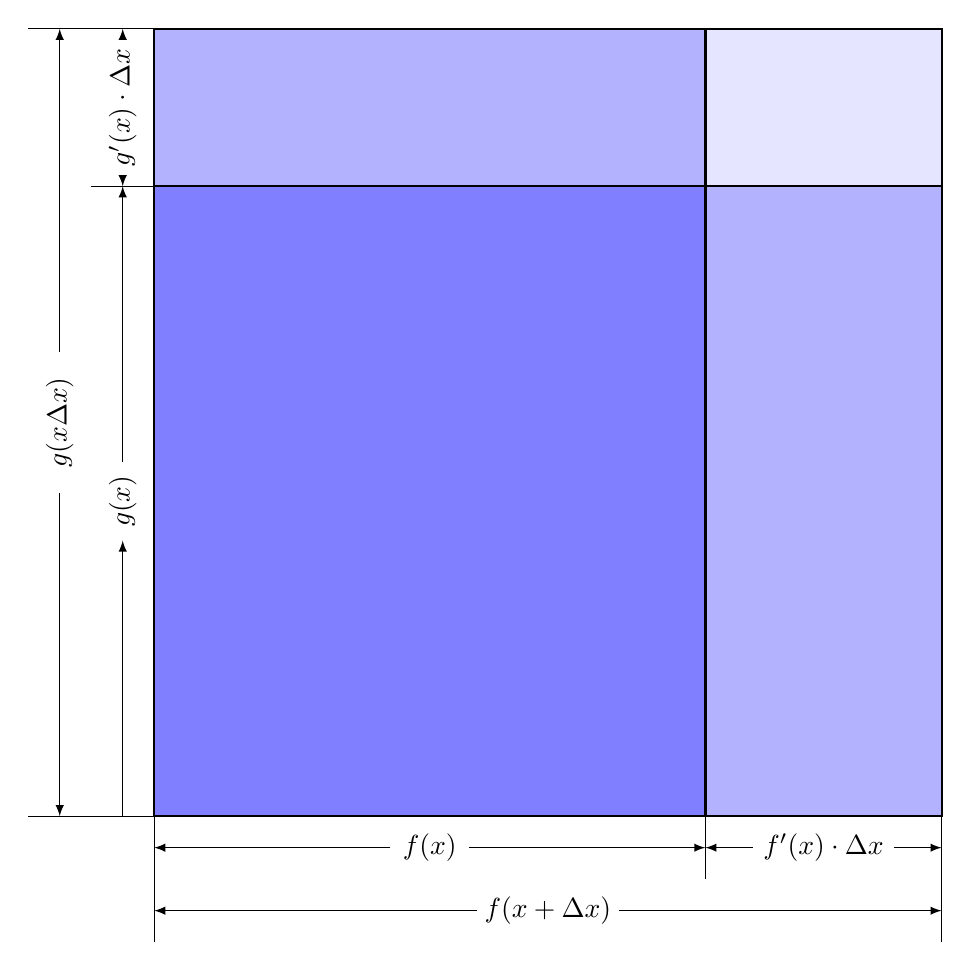
\begin{tikzpicture}[scale=2]
	\fill[blue,opacity=0.5] (0,0)rectangle(3.5,4);
	\fill[blue,opacity=0.3] (0,4)rectangle(3.5,5);
	\fill[blue,opacity=0.3] (3.5,0)rectangle(5,4);
	\fill[blue,opacity=0.1] (3.5,4)rectangle(5,5);
	\draw[-,thick] (0,0)--(5,0)--(5,5)--(0,5)--(0,0);
	\draw[-] (0,0)--(-0.4,0);
	\draw[-] (0,4)--(-0.4,4);
	\draw[-] (0,5)--(-0.5,5);
	\draw[-,thick] (0,4)--(5,4);
	\draw[-,thick] (3.5,0)--(3.5,5);
	\draw[-] (0,0)--(0,-0.8);
	\draw[-] (3.5,0)--(3.5,-0.4);
	\draw[-] (5,0)--(5,-0.8);
	\node at (1.75,-0.2) {$f(x)$};
	\node at (4.25,-0.2) {$f'(x)\cdot\Delta x$};
	\node at (2.5,-0.6) {$f(x+\Delta x)$};
	\draw[-latex] (1.5,-0.2)--(0,-0.2);
	\draw[-latex] (2,-0.2)--(3.5,-0.2);
	\draw[-latex] (3.8,-0.2)--(3.5,-0.2);
	\draw[-latex] (4.7,-0.2)--(5,-0.2);
	\draw[-latex] (2.05,-0.6)--(0,-0.6);
	\draw[-latex] (2.95,-0.6)--(5,-0.6);
	\draw[-] (0,0)--(-0.8,0);
	\draw[-] (0,5)--(-0.8,5);
	\draw[-] (0,4)--(-0.4,4);
	\node[rotate=90] at (-0.2,2) {$g(x)$};
	\node[rotate=90] at (-0.2,4.5) {$g'(x)\cdot\Delta x$};
	\node[rotate=90] at (-0.6,2.5) {$g(x\Delta x)$};
	\draw[-latex] (-0.6,2.05)--(-0.6,0);
	\draw[-latex] (-0.6,2.95)--(-0.6,5);
	\draw[-latex] (-0.2,0)--(-0.2,1.75);
	\draw[-latex] (-0.2,2.25)--(-0.2,4);
	\draw[-latex] (-0.2,4.95)--(-0.2,5);
	\draw[-latex] (-0.2,4.05)--(-0.2,4);
\end{tikzpicture}
\end{document}
\end{document}